\chapter{Implementation}
%Only the final state of the implementation should be described: not a blow by blow history of its development. However, each of the major design decisions should be identified and reasons given for the choices made. You should abstract away from the code and outline the overall structure of the system and the key algorithms in abstract form, e.g. using diagrams or formalised English. You can point to bits of actual code in the appendices, if necessary. A worked example is often helpful.

In this chapter, we will explain and motivate the design of our system, and go over the procedures for evaluation of the system.
The chapter starts with an overview of the structure of the data together with a description of how the data was processed and cleaned for use by our system.
Next, a brief overview of the data exploration stage, detailing different structures of the data and comparing the different data sets created, is given.
Following this, the loss function, and the different metrics it is constructed of, is presented.
It is shown how all metrics together help fulfill all constraints outlined in \cref{sec:aim}.
Finally, the constructions of the models are explained one by one, with the focus being on GERT, the model introduced in this thesis.


\label{sec:method}
% The methodology chapter describes how the work is structured. It includes workflows, design of experiments and use of various data collection methods. Ideally, a methodology chapter should be sufficiently detailed that anyone with certain basic knowledge of the field should be able to carry out the work in the way described in the report and achieve the same results. Describing the methodology is an important factor in enabling the company offering the assignment, to assess whether or not the goal can be achieved as described. It is therefore also important to explain why the chosen methodology offers a reliable outcome.

\begin{figure}
    \centering
    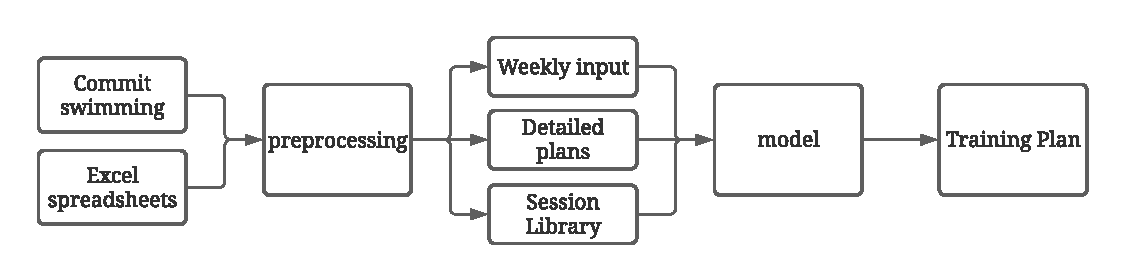
\includegraphics[width=1.0\linewidth]{chapters/figures/implementation_plots/data_pipeline_workflow.pdf}
    \caption{A flowchart illustrating the data pipeline from raw data to a finished training plan}
    \label{fig:data_pipeline}
\end{figure}

%
\section{Data Cleaning and Preprocessing}
\label{sec:data}
A library of 5313 historical training sessions and self-reported de-identified training logs for athletes trained by a professional coach was supplied by the company SVEXA. 
The logs contain detailed information for each training session. 
The data was supplied in two different formats.
All data from before September 2019 was stored in excel spreadsheets while data after that was stored in Commit Swimming\footnote{\href{https://commitswimming.com/}{Link to the Homepage of Commit Swimming}} in JSON format.
As a first step, the data from both sources were extracted and reformatted to fit into a Pandas dataframe\footnote{\href{https://pandas.pydata.org/pandas-docs/stable/reference/api/pandas.DataFrame.html}{Link to Pandas Documentation of the DataFrame Type}}.

The dataframe, hereinafter referred to as the \textit{session library}, contains information about the volume swum in different intensity zones, a detailed description of the session performed and additional meta-information on the type of the main set of the session as well as what competition type, also known as specialty, see \cref{tab:session_specialties}, the session is suited for.
A description of the format of a session in the session library can be seen in \cref{tab:session_lib_description}.

\begin{table}
\centering
\begin{tabularx}{0.9\textwidth}{lL}
\toprule
Specialty & Description \\ 
\midrule
Sprint    & A workout for athletes specializing in shorter distances, such as 50- and 100m events. \\
Middle    & A workout for athletes specializing in middle distances, such as 200- and 400m events. \\
Long      & A workout for athletes specializing in events longer than 400m. \\
\bottomrule
\end{tabularx}
\caption{A table describing the different specialties of sessions in the session library. Note that even though an athlete is specialized in a certain distance it is possible to compete in other events.}
\label{tab:session_specialties}
\end{table}

\begin{table}
\centering
\begin{tabularx}{0.9\textwidth}{lL}
\toprule
Property  & Description                                                 \\ \midrule
Label     & The type of training session                                \\
I-II      & Training load accumulated in zone 1 and 2                   \\
...       & ...                                                         \\
VII       & Training load accumulated in zone 8                         \\
Specialty & The specialty for which the session is suitable             \\
Detail    & A detailed description of what training should be performed \\ \bottomrule
\end{tabularx}
\caption{A table showing the descriptions of the properties of the sessions in the session library.}
\label{tab:session_lib_description}
\end{table}

The data was self-reported which made it necessary to clean.
The data set was, however, already very limited in terms of the amount of data.
Since the goal was to produce weekly plans, it was deemed a better alternative to keep weeks with faulty data points by just removing the faulty session rather than removing the whole week's worth of data, even though this altered the week itself.
It was assumed that the faulty sessions were uniformly random distributed and the model would therefore still be able to learn the underlying distributions despite the added noise.

The cleaning process started with the removal of all obviously malformed data, such as negative or absurdly large amounts of training together with all empty sessions and all sessions where training had been disturbed by travel, sickness, competitions or similar.
Secondly, for every session, the predominant intensity zone was used as a proxy to assign new labels, since the original labels were erroneous at times.
A description of these labels can be seen in table \cref{tab:session_labels}.
It is worth noting that since intensity zones III and IV were reported together, it was not possible to distinguish between aec2 and aec3 type sessions.
Consequently, these were grouped into a single label called aec23.
Finally, the data was labelled with unsupervised outlier detection using local outlier factor which flagged training sessions that differed from the rest of the sessions.\footnote{\href{https://scikit-learn.org/stable/modules/generated/sklearn.neighbors.LocalOutlierFactor.html}{Link to Scikit Learn's Documentation on Local Outlier Factor}}
These sessions were also removed as they were thought to be misreported.

\begin{table}
\centering
\begin{tabularx}{0.9\textwidth}{llL}
\toprule
Label  & Intensity Zone & Description                                                             \\ \midrule
rest   & 0              & Rest                                                                    \\
aec1   & II             & Aerobic capacity, builds aerobic base through long distance training    \\
aec23  & III-IV         & Aerobic and anaerobic threshold training and intensive endurance training. \\
aep    & V              & Aerobic power and aerobic effect, training at lactic threshold          \\
anp    & VI             & Anaerobic power, races or training at race pace                         \\
anc    & VII            & Anaerobic capacity, power development                                   \\
alac   & VIII           & Alactic sprint, training of top speed, starts and turns                \\ \bottomrule
\end{tabularx}
\caption{A table describing the different types of sessions in the session library. Note that since intensity zones III and IV were reported as a single unit in the data, it was not possible to distinguish between aec2 and aec3 type sessions. Consequently, these were grouped into a single label called aec23.}
\label{tab:session_labels}
\end{table}


The cleaned session data was then aggregated to complete training weeks.
During this aggregation, it was assumed that the athletes trained at most two sessions in the pool per day, which holds for almost all days.
For the instances where it did not hold, only the first two sessions were used in the aggregation.
The assumption was introduced to simplify the problem, making the solution space enumerable.
The aggregated weekly data was also cleaned using local outlier factor to identify and remove abnormal weeks.
This can seem out of line with our goal of preserving as many weeks as possible.
However, as can be seen in \cref{fig:outlier_motivation} some weeks were still, despite the earlier cleaning and correction efforts, in the realm of improbability and needed to be removed.
This was the last stage where any data was removed and the remaining library of training sessions now contained $2702$ sessions.
\begin{figure}[ht]
    \centering
    \begin{subfigure}[t]{0.48\textwidth}
        \centering
        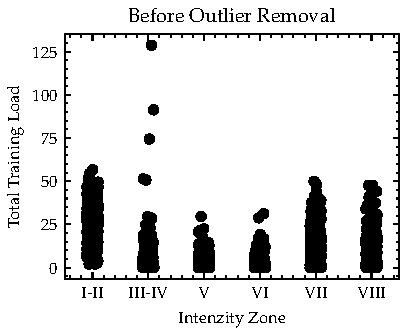
\includegraphics[width=\textwidth]{chapters/figures/implementation_plots/before_outlier_removal.pdf}
        % \captionsetup{width=.9\linewidth}
        % \caption{Number of sessions per week}
    \end{subfigure}%
    ~ 
    \begin{subfigure}[t]{0.48\textwidth}
        \centering
        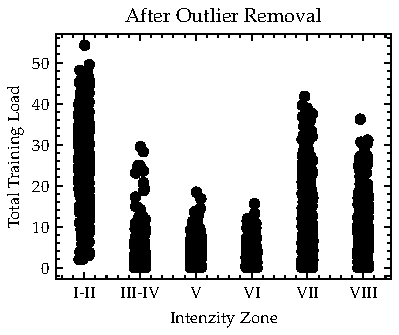
\includegraphics[width=\textwidth]{chapters/figures/implementation_plots/after_outlier_removal.pdf}
        % \captionsetup{width=.9\linewidth}
        % \caption{Volume per week}
    \end{subfigure}
        \caption{Strip plots of the total training load for each week before (left) and after (right) outlier detection and removal was run.}
    \label{fig:outlier_motivation}
\end{figure}

Next, the aggregated weekly data was split into two parts.
The first part, called \textit{weekly input}, consists of the data about the athlete (age, gender, specialty), goals (weeks left of macrocycle, focus area, weekly training load per intensity zone), and schedule constraints (number of sessions per week).
The second part, called \textit{detailed plans}, consists of a sequence of sessions that corresponds to the training performed for a week in \textit{weekly input}.

Lastly, the data was randomly sampled into an 80-20 train-test split in three different ways, which are illustrated in \cref{fig:random_splits}.
First, a train-test split was created by sampling random data points (pairs of elements from \textit{weekly input} and \textit{detailed plans}).
% This is the set that was used for parameter tuning for the GERT model that is described in \cref{sec:GERT}.
Second, the data was split into train- and test sets based on randomly sampled calendar weeks.
The reasoning behind this was that athletes often train together in groups. 
Therefore, another athlete could have performed the same sessions, which might affect the performance of the model.

Third, a held-out data set of an entire macrocycle spanning from August through November of 2020 for all athletes was created.
These were also the chronologically last points in the data set and were therefore chosen as a representation of what an actual user scenario would look like.
It is, however, worth mentioning that at the time of this thesis the world was in the covid-19 pandemic. 
It is therefore not certain that these data points are representative of what a usual training cycle would look like.

\begin{figure}[ht]
    \centering
    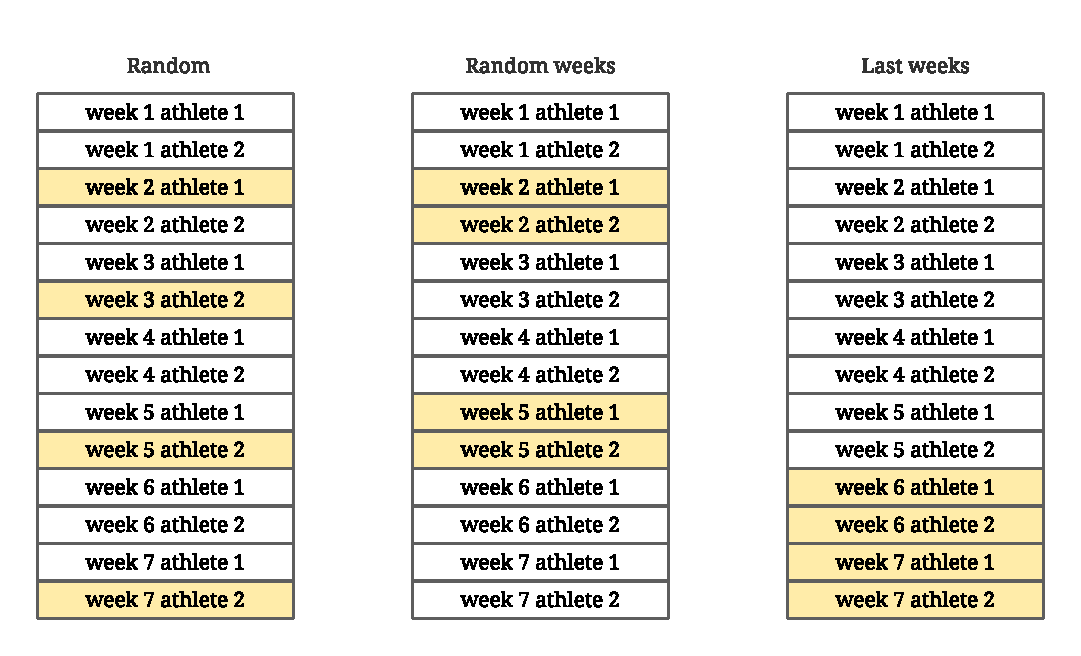
\includegraphics[width=\textwidth]{chapters/figures/implementation_plots/random_split_illustration.pdf}
    \caption{An illustration of the different ways the data set was split into train- and test sets. The samples that are chosen for the test set are marked with yellow.}
    \label{fig:random_splits}
\end{figure}

\section{Data Exploration}
Once the data was cleaned, processed and split into different data sets, an exploration of the data was made. 
Firstly, the distributions of the number of sessions and volume per week for the whole data set were investigated.
Histograms of these distributions can be seen in \cref{fig:data_exploration_histograms}.
Most training weeks have between 5 and 10 training sessions and the swimmers accumulate \SIrange{10}{50}{\kilo\meter} of swimming per week.


\begin{figure}[ht]
    \centering
    \begin{subfigure}[t]{0.48\textwidth}
        \centering
        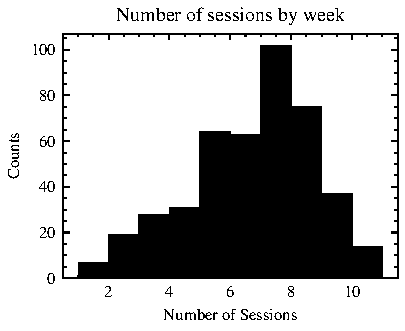
\includegraphics[width=\textwidth]{chapters/figures/data_exploration/hist_nbr_sessions.pdf}
        % \captionsetup{width=.9\linewidth}
        % \caption{Number of sessions per week}
    \end{subfigure}%
    ~ 
    \begin{subfigure}[t]{0.48\textwidth}
        \centering
        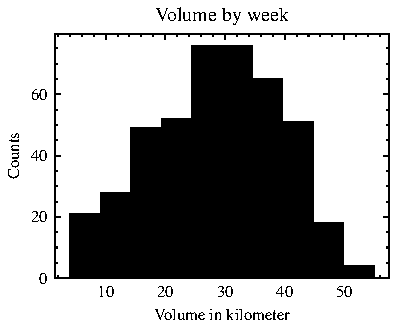
\includegraphics[width=\textwidth]{chapters/figures/data_exploration/hist_volume.pdf}
        % \captionsetup{width=.9\linewidth}
        % \caption{Volume per week}
    \end{subfigure}
    \caption{Histograms of the number of training sessions (left) and volume per week (right) for the data set.}
    \label{fig:data_exploration_histograms}
\end{figure}

Next, the distribution of the total training load for a week was investigated.
The mean total training load for all three splits was found to be around 50 and they were all similarly distributed, which is expected.
Histograms showing the training data for the different splits can be seen in \cref{fig:data_exploration_split_histogram}

\begin{figure}[ht]
    \centering
    \begin{subfigure}[t]{0.48\textwidth}
        \centering
        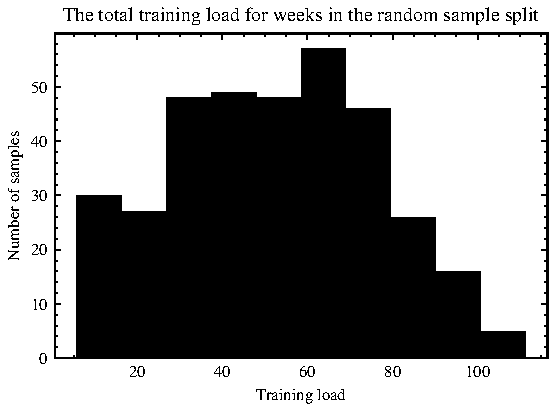
\includegraphics[width=\textwidth]{chapters/figures/data_exploration/random_sample_hist.pdf}
        \captionsetup{width=.9\linewidth}
        \caption{Random samples split}
    \end{subfigure}%
    ~ 
    \begin{subfigure}[t]{0.48\textwidth}
        \centering
        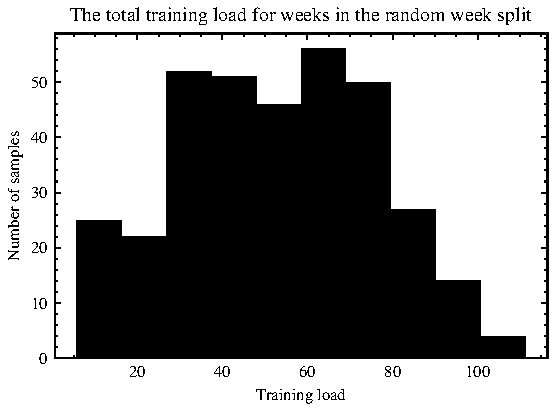
\includegraphics[width=\textwidth]{chapters/figures/data_exploration/random_week_hist.pdf}
        \captionsetup{width=.9\linewidth}
        \caption{Random week split}
    \end{subfigure}\\[1ex]
    \begin{subfigure}[t]{0.48\textwidth}
        \centering
        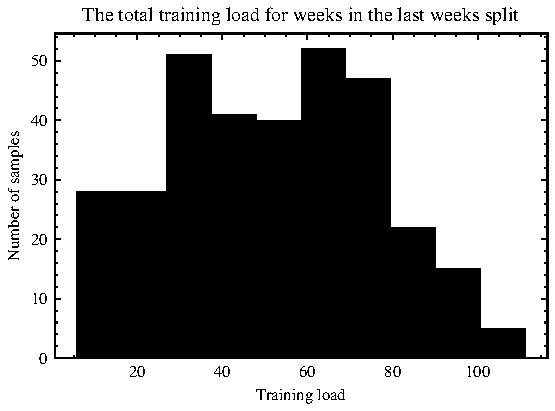
\includegraphics[width=\textwidth]{chapters/figures/data_exploration/last_weeks_hist.pdf}
        \captionsetup{width=.9\linewidth}
        \caption{Last weeks split}
    \end{subfigure}
    \caption{Histograms showing the distribution of total training load for each week for the three different splits.}
    \label{fig:data_exploration_split_histogram}
\end{figure}

Further, the distribution of training load over the different sessions was investigated.
Same as for the total training load, the distributions for the different splits were similar to each other. 
As can be seen in \cref{fig:data_exploration_distribution} the athletes typically follow a pattern of resting or lighter training on sessions $6$ and $12$-$14$, with varied, more heavy training in between.
Interleaving rest days with the training in a fairly static pattern is expected since the athletes need to recover between training sessions.

\begin{figure}[ht]
    \centering
    \begin{subfigure}[t]{0.48\textwidth}
        \centering
        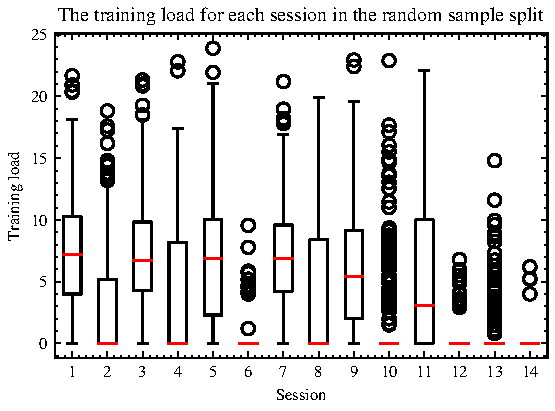
\includegraphics[width=\textwidth]{chapters/figures/data_exploration/random_sample_session_boxplot.pdf}
        \captionsetup{width=.9\linewidth}
        \caption{Random samples split}
    \end{subfigure}%
    ~ 
    \begin{subfigure}[t]{0.48\textwidth}
        \centering
        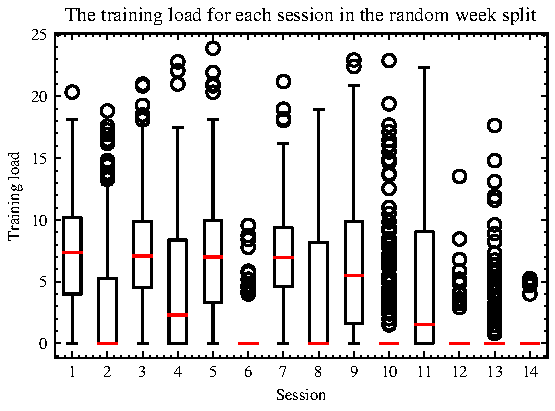
\includegraphics[width=\textwidth]{chapters/figures/data_exploration/random_week_session_boxplot.pdf}
        \captionsetup{width=.9\linewidth}
        \caption{Random week split}
    \end{subfigure}\\[1ex]
    \begin{subfigure}[t]{0.48\textwidth}
        \centering
        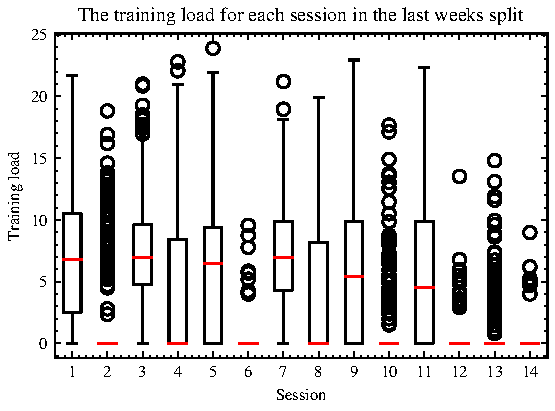
\includegraphics[width=\textwidth]{chapters/figures/data_exploration/last_weeks_session_boxplot.pdf}
        \captionsetup{width=.9\linewidth}
        \caption{Last weeks split}
    \end{subfigure}
    \caption{Box plots showing the distribution of total training load for each session in the week for the three different splits.}
    \label{fig:data_exploration_distribution}
\end{figure}

Also, the amount of training load in the different intensity zones was investigated.
As can be seen in \cref{fig:data_exploration_zones} athletes typically perform most of their swimming at lower intensities.
This is complemented by high-intensity sessions while swimming at moderate intensities is not as common.
This split is common to see in the training of endurance athletes.
A well-known heuristic is to have an \SIrange{80}{20}{\percent} distribution of volume between low and high-intensity training.

\begin{figure}[ht]
    \centering
    \begin{subfigure}[t]{0.48\textwidth}
        \centering
        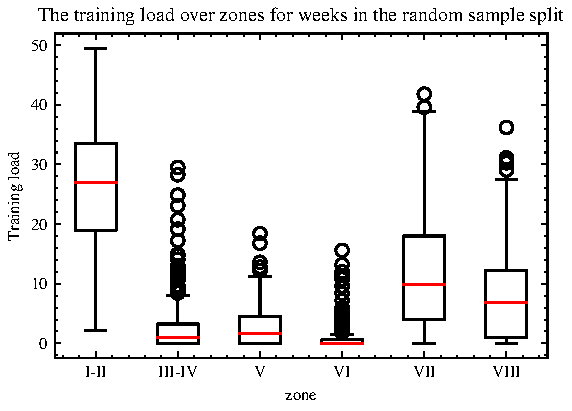
\includegraphics[width=\textwidth]{chapters/figures/data_exploration/random_sample_zone_boxplot.pdf}
        \captionsetup{width=.9\linewidth}
        \caption{Random samples split}
    \end{subfigure}%
    ~ 
    \begin{subfigure}[t]{0.48\textwidth}
        \centering
        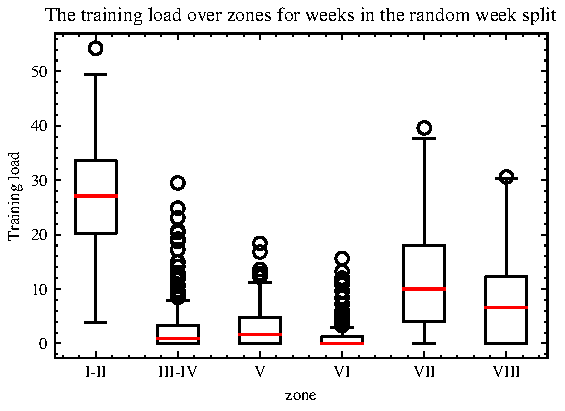
\includegraphics[width=\textwidth]{chapters/figures/data_exploration/random_week_zone_boxplot.pdf}
        \captionsetup{width=.9\linewidth}
        \caption{Random week split}
    \end{subfigure}\\[1ex]
    \begin{subfigure}[t]{0.48\textwidth}
        \centering
        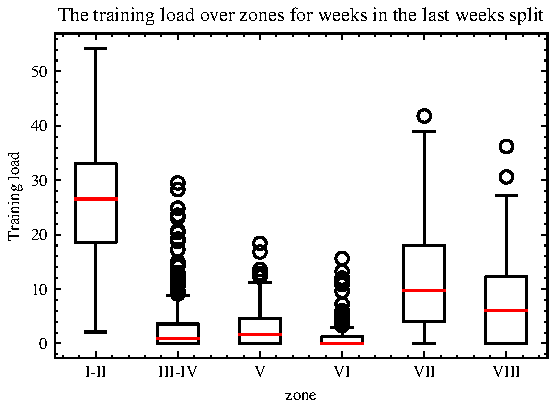
\includegraphics[width=\textwidth]{chapters/figures/data_exploration/last_weeks_zone_boxplot.pdf}
        \captionsetup{width=.9\linewidth}
        \caption{Last weeks split}
    \end{subfigure}
    \caption{Box plots showing the distribution of training load over the intensity zones for the three different splits.}
    \label{fig:data_exploration_zones}
\end{figure}

Finally, the difference between the athletes that specialize in different events was investigated.
As can be seen in \cref{fig:data_exploration_spec}, the distribution of training load over the different sessions of the week was found to be almost identical for the different specializations. 
There was, however, a difference in the types of sessions and distribution over intensity zones.
Athletes that specialize in middle distance races typically performed more swimming in zones $IV-VI$.
This also made intuitive sense since the middle distance athletes compete in longer races, and therefore need to tolerate work for longer periods of time, which is trained by the work in these zones.
The difference in types of session performed naturally follows since the labels were inferred from intensity zones.


\begin{figure}[ht]
    \centering
    \begin{subfigure}[t]{0.48\textwidth}
        \centering
        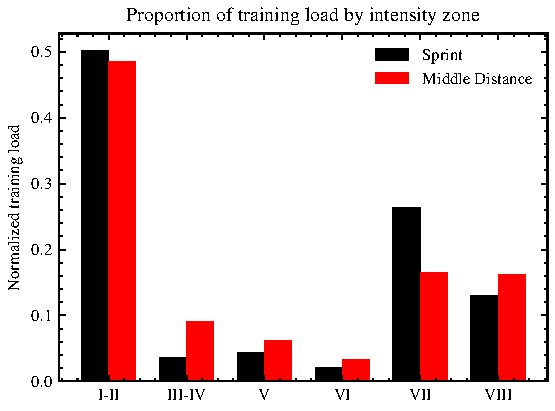
\includegraphics[width=\textwidth]{chapters/figures/data_exploration/tl_by_intensity_spec.pdf}
        \captionsetup{width=.9\linewidth}
        \caption{Intensity zones}
    \end{subfigure}%
    ~ 
    \begin{subfigure}[t]{0.48\textwidth}
        \centering
        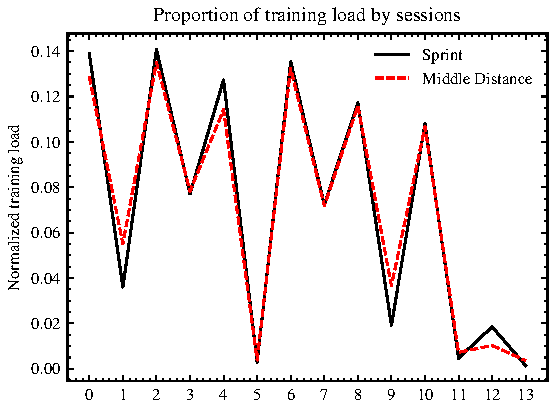
\includegraphics[width=\textwidth]{chapters/figures/data_exploration/tl_by_session_spec.pdf}
        \captionsetup{width=.9\linewidth}
        \caption{The training load distribution over different sessions of the week}
    \end{subfigure}\\[1ex]
    \begin{subfigure}[t]{0.48\textwidth}
        \centering
        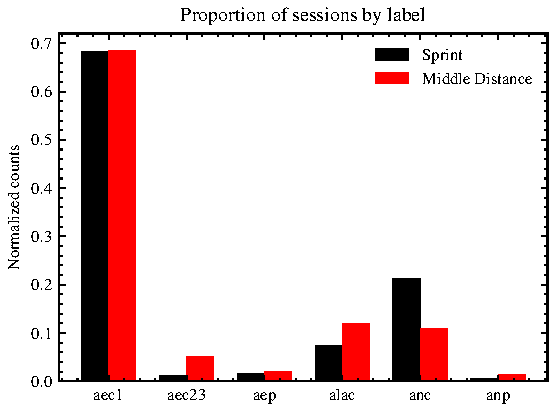
\includegraphics[width=\textwidth]{chapters/figures/data_exploration/labels_by_spec.pdf}
        \captionsetup{width=.9\linewidth}
        \caption{The proportion of sessions of each type}
    \end{subfigure}
    \caption{Plots showing the differences between athletes with different specialties for intensity distribution, weekly distribution, and the types of sessions performed.}
    \label{fig:data_exploration_spec}
\end{figure}
% Check difference over specialty
% Frequencies for different session types


\section{Metrics}
One of the main challenges with this study is how to evaluate the results.
What metrics can be used to compare the likeness of two training plans?
% There are two main considerations for determining the likeness of training plans.
% Firstly, there is the aspect of contents.
% Does the generated training plan contain sessions that are similar to what the coach would produce?
% Secondly, there is the aspect of ordering.
% Are the generated sessions placed in an order similar to how the coach would have placed them?
The objectives specified in \cref{sec:aim} serve as motivation and a target for all metrics presented in this section.

The objectives specified in \cref{sec:aim} can also be reconsidered as constraints that can be used during optimization.
Optimization constraints are considered to be in one of the two groups hard- or soft constraints.
Hard constraints are the constraints that must be satisfied by all feasible solutions, while soft constraints are to be optimized for in the space of feasible solutions.
This work will consider \cref{constraint:tl_total,constraint:tl_week,constraint:tl_zones,constraint:order} to outline soft constraints while \cref{constraint:types,constraint:specialty} outline hard constraints. 
 
The soft constraints can be incorporated by the use of three error functions.
First, we look at the total training load in each intensity zone.
Given the training loads for the coach's training plan, $Y_{ij}>=0$, and the model-created training plan, $\hat{Y}_{ij}>=0$, where $i \in S := \{\mathrm{sessions}\}$, $j \in Z := \{\mathrm{intensity\ zones}\}$ , we calculate the quadratic mean of the difference of total training load over all intensity zones. That is 
\begin{equation}
    e_{Z} = \sqrt{\frac{1}{|S|}\sum_{i \in S}\left(\sum_{j \in Z}\hat{Y}_{ij}-Y_{ij}\right)^2}\,.
\end{equation}
When optimized for, this metric helps to fulfill \cref{constraint:tl_total,constraint:tl_zones}, similar total training load and similar distribution of training load over the intensity zones.

Second, we look at the distribution of training load over the sessions.
For this, we calculate the quadratic mean of the difference of total training load over all sessions. That is 
\begin{equation}
    e_{D} = \sqrt{\frac{1}{|Z|}\sum_{j \in Z}\left(\sum_{I \in S}\hat{Y}_{ij}-Y_{ij}\right)^2}\,.
\end{equation}
When optimized for, this metric helps to fulfill \cref{constraint:tl_total,constraint:tl_week}, similar total training load and similar distribution of training load over the sessions.

Third, defining \textit{triplet} as subsequences of length three, we look at the cardinality of the symmetric difference between the set of triplets of session types from the model-created training plan and the set of triplets of session types from the coach's training plan.
That is, given the session type indicators for the coach's training plan, $Y_{ik}$, and the model-created training plan, $\hat{Y}_{ik}$, where $i \in S := \{\mathrm{sessions}\}$, $k \in T := \{\mathrm{session\ types}\}$, and 
\begin{equation*}
    Y_{ik} = \begin{cases}
    1, & \text{if session $i$ is of type $k$}   \\
    0, & \text{otherwise}
    \end{cases},
\end{equation*} 
create the sets
$$U:=\{(Y_{(i-1)k},\ Y_{ik},\ Y_{(i+1)k}) : i-1\in S,\ i+1\in S \}\,,$$
$$C:=\{(\hat{Y}_{(i-1)k},\ \hat{Y}_{ik},\ \hat{Y}_{(i+1)k}) : i-1\in S,\ i+1\in S \}$$
and calculate the cardinality of their symmetric difference as
\begin{equation}
    e_T = \frac{1}{2}|C\bigtriangleup U|\,.
\end{equation}
When optimized for, this error function helps to fulfill \cref{constraint:order}, similar ordering of session types.
The constant $1/2$ is so that the metric is consistent with the intuitive notion of the number of differing triplets between the sessions.
This metric will for example produce a high score if the sessions of the plans are reversed or individually swapped around, but a low score if they are ordered similarly, or only large or similar sequences are swapped.

For the hard constraints, we opted to use relaxations, creating error functions that could be heavily penalised during optimization.
This made the hard constraints possible to incorporate using two error functions.
First, we look at the types of training sessions for both training plans.
Given the type indicators for the sessions for the coach's training plan, $Y_{ik}$, and the model-created training plan, $\hat{Y}_{ik}$, where $i \in S := \{\mathrm{sessions}\}$, $k \in T := \{\mathrm{session\ types}\}$, and 
\begin{equation*}
    Y_{ik} = \begin{cases}
    1, & \text{if session $i$ is of type $k$}   \\
    0, & \text{otherwise}
    \end{cases},
\end{equation*} 
we calculate the number of sessions where the type differ between the plans as
\begin{equation}
    e_{F} = \frac{1}{2}\sum_{k \in T}\left|\sum_{i \in S}\hat{Y}_{ik}-Y_{ik}\right| \,.
\end{equation}
When optimized for, this metric helps to fulfill \cref{constraint:types}, same number of each session type. 

Second, we look at what specialties the sessions in the plans are suited for.
Given the specialty indicators for the sessions for the coach's training plan, $Y_{il}$, and the model-created training plan, $\hat{Y}_{il}$, where $i \in S := \{\mathrm{sessions}\}$, $l \in D := \{\mathrm{Specialties}\}$, and 
\begin{equation*}
    Y_{il} = \begin{cases}
    1, & \text{if session $i$ is suited for specialty $l$}   \\
    0, & \text{otherwise}
    \end{cases},
\end{equation*} 
we calculate the number of sessions where the specialty differ between the plans as
\begin{equation}
    e_{S} = \frac{1}{2}\sum_{l \in D}\left|\sum_{i \in S}\hat{Y}_{il}-Y_{il}\right| \,.
\end{equation}
When optimized for, this metric helps to fulfill \cref{constraint:specialty}, same number of each specialty session. 

To be able to fulfill all constraints simultaneously, optimization was done for the soft constraints while first prioritising the hard constraints, the loss function,
\begin{equation}
    \mathcal{L} = \left(\left( c_1 e_{Z}\right)^2 + \left( c_2 e_{D}\right)^2 + \left( c_3 e_{T}\right)^2 + \left( c_4 e_{F}\right)^2 + \left( c_5 e_{S}\right)^2\right)^{1/2} \,,
    \label{eq:loss_func}
\end{equation}
with $c_1=c_2=c_3=1$ and $c_4=c_5=100$, was created.
$c_1$ to $c_5$ were set to \num{1} and \num{100} to ensure that all soft constraints were considered equally and all hard constraints equally, while the hard constraints always would be prioritised over the soft.

\section{GERT}
\label{sec:GERT}
We introduce the Genetic and Random Trees training planner (GERT) that consists of two modules: a machine learning system trained to infer a weekly load distribution and order of sessions, and a planning system that constructs a detailed plan of individual sessions selected from the session library (implemented as a genetic algorithm \cite{whitley1994genetic}).
An overview of GERT's structure can be seen in \cref{fig:GERT_overview}.

\begin{figure}[ht]
    \centering
    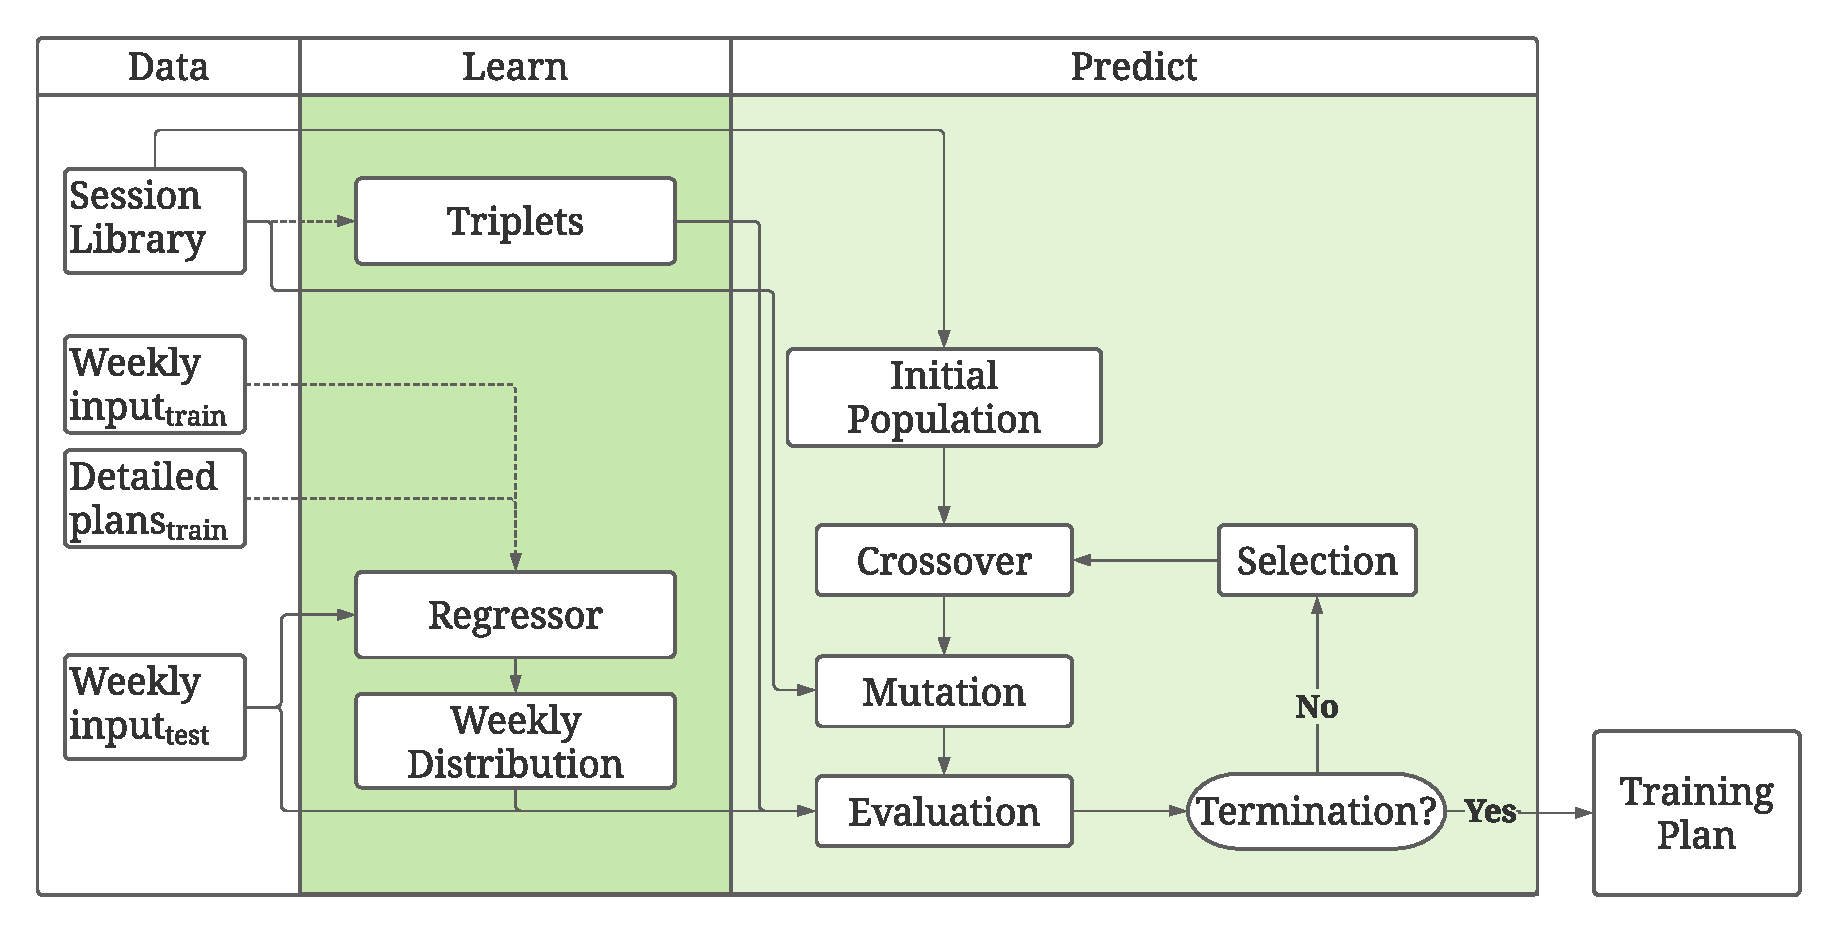
\includegraphics[width=1.0\linewidth]{chapters/figures/implementation_plots/GERT_overview.pdf}
    \caption{An overview of GERT. In the left column labeled \textit{Data} all inputs to GERT are listed. In the middle column labeled \textit{learning} all stages used during the \textit{Learning the coach's style} portion of the model execution is listed. The dotted arrows represent the data flow during this execution portion.
    In the right column labeled \textit{Prediction} all stages used during the \textit{Generating training plans} portion of execution are listed. The full arrows represent the data flow during this execution portion.}
    \label{fig:GERT_overview}
\end{figure}

\subsection{Learning the coach's style}
The first action of the GERT model is to extract, from historical data, how a coach would create a training plan given \textit{weekly input}.
This is done in two steps. 
First, an internal regression model is fitted to the distribution of training load over the sessions in the historical training plans.
Secondly, a database of consecutive triplets of session types is created from the historical plans.

To estimate the distribution of training load over the sessions GERT uses a random forest regressor chain described in \ref{sec:regressor_chain}.
The regressor tries to predict the weekly distribution of training load, that is how much of the total training of the week should be done each session, with the goal of minimizing the quadratic mean of the differences between the prediction and true distribution.
This metric is also known as the Root Mean Squared Error, RMSE, which is the shorthand that will be used here.

Further, the regressor will try to predict the total training load, rather than the training load of each intensity zone. 
This reduces the number of output variables to be predicted from $84$ (14 sessions and 6 intensity zones) to $14$, which further reduces the training time, prediction time and overall complexity of the model.

The regressor can not coordinate perfectly between the outputs to make sure that constraints for the correct number of sessions and total training load, \cref{constraint:tl_total,constraint:types}, are upheld.
This is remedied by removing the sessions with the lowest inferred training load from the predicted distribution so that the output had the specified number of sessions, and then re-scaling the output to have the total training load as specified.
The regressor pipeline is illustrated in \cref{fig:regressor_illustration}.

\begin{figure}
    \centering
    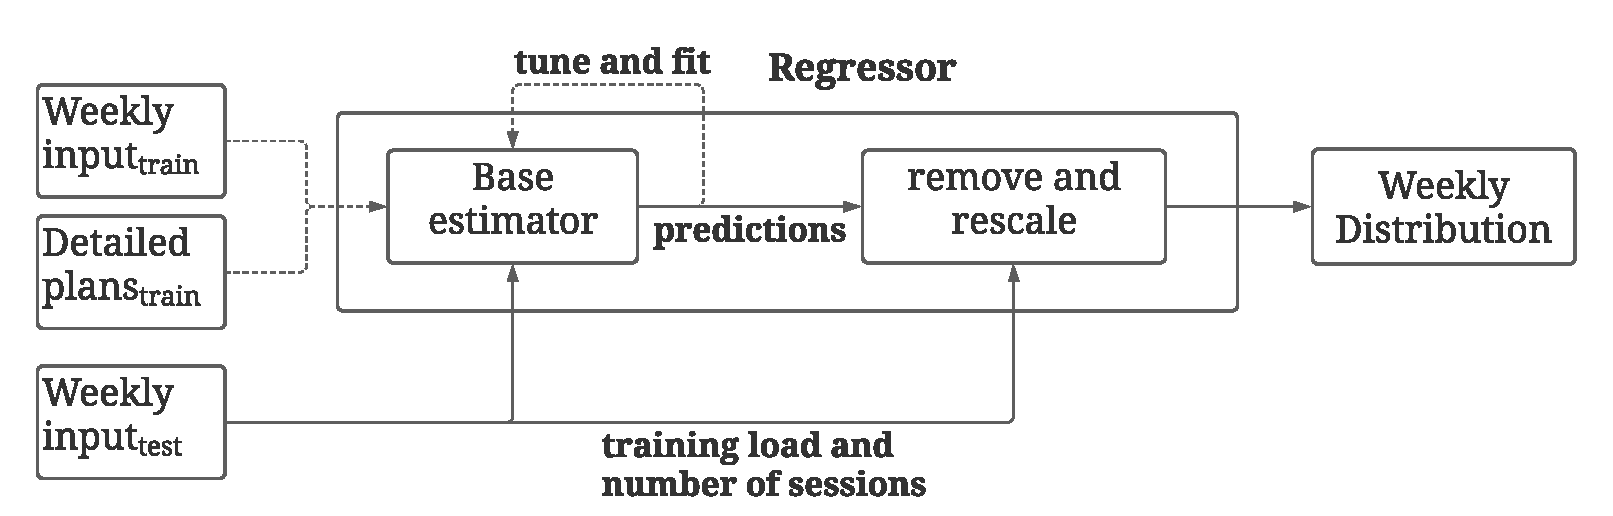
\includegraphics[width=0.8\linewidth]{chapters/figures/implementation_plots/regressor_illustration.pdf}
    \caption{An illustration of the regressor for the weekly distribution.
    The base estimator (random forest regressor chain) is trained and tuned in isolation, the predictions are then rescaled to fit the GERT algorithm. }
    \label{fig:regressor_illustration}
\end{figure}

% The task of predicting the distribution over the sessions was a multi target regression problem.
% This was approached in two different ways.
% Firstly, a naive approach was taken, where each output was considered to be independent and one regressor was trained for each output variable.
% Secondly, regressor chains were implemented according to \cref{sec:regressor_chain}.
% However, both of these approaches suffer from the same problem.

To choose the regressor that should be included in GERT, we tested different regressors using five-fold cross-validation on the training data.
The outputs from the tuned regressors were edited according to the procedure described above and evaluated using cross-validation.
The results from the top 5 models can be seen in \cref{tab:weekly_cv_results}
The random forest regressor chain was the best performing model.
Consequently, this model was chosen as the regressor component in the GERT model.

\begin{table}
    \centering
    \begin{tabularx}{0.7\textwidth}{lrr}
    \toprule
                          model & $RMSE$ &  std \\
    \midrule
          RandomForestRegressor &  3.59 &  0.17 \\
             ExtraTreesRegressor &  3.57 &  0.12 \\
                 ElasticNetChain &  3.61 &  0.16 \\
      \textbf{RandomForestRegressorChain} &  \textbf{3.54}&  \textbf{0.13} \\
        ExtraTreesRegressorChain &  3.58 &  0.15 \\
    \bottomrule
    \end{tabularx}
    \caption{Results from the top 5 regressors from the 5-fold cross-validation of the weekly distribution regressors. A lower RMSE is better.}
    \label{tab:weekly_cv_results}
\end{table}

To learn which order the sessions should be placed in, GERT constructs a database of triplets of training types to use as a proxy for how the coach would typically order the different session types.
The choice to look at triplets, sequences of length three, is based on the probability of observation. 
With the $7$ session types that are described in \cref{tab:session_labels}, there are $7^3=343$ possible unique triplets that could be observed.
Per week, sequence of $14$ sessions, there can be at most $12$ unique triplets identified.
For a training set of about $350$ weeks, this results in $4200$ observed triplets.
This gives a good chance of having observed most of the triplets the coach would use since the set of observed triplets is roughly $12$ times larger than the set of possible unique triplets.
The same calculation for continuous sequences of length four, however, reveals that the total number of possible unique sequences, $7^4=2401$, is more than half of the maximum number of sequences possible to observe.
This ratio is far too small for it to be considered likely to have observed most of the allowed sequences.


\subsection{Generating training plans}
The goal of this stage is to generate a training plan based on sessions from the session library such that the objectives specified in \cref{sec:aim} are fulfilled.
To accomplish this, we develop a genetic algorithm inspired by Whitley \cite{whitley1994genetic}.

The first step of our genetic algorithm is to create a random initial population where the size of the population is specified as a hyperparameter to the model.
The population is created by randomly sampling the specified number of sessions from the session library and distributing them randomly over the week.

In contrast to canonical genetic algorithms described in \cref{sec:genetic_algorithms}, a fitness score is not calculated as a first step after creating the initial population to decide which samples should go on to an intermediate population.
Instead, all samples are considered equally for both crossover and mutation.
The population is also expanded until the selection stage of the algorithm, instead of replaced as in the canonical algorithm.
These changes are made because both what sessions are chosen from the library and in what order they are placed, are of importance and allows a training plan which has the right sessions in the wrong order to be shuffled before its fitness score is calculated, potentially saving it from removal.

Next, children are added to the population by recombining samples from randomly selected parents using uniform crossover, described in section \cref{sec:genetic_algorithms}.
Mutation is performed on copies of all samples with the probability of mutation set as a hyperparameter.
Two variations of mutation are performed.
First, a random session from the plan can be replaced entirely by another random session from the library.
Second, the order of the sessions of the plan can be randomly shuffled.
After this, the mutated samples are added to the population as well.

When crossover and mutation have been performed, a fitness score is calculated for each training plan using the loss function from \cref{eq:loss_func}.
To be able to evaluate the terms $e_D$ and $e_T$ of the loss function, the regression model and the database of historical sequences of training types are used. 
An illustration of how a training plan is evaluated in terms of $e_D$ and $e_Z$, corresponding to objectives \cref{constraint:tl_week,constraint:tl_zones}, that the generated week has the right distribution over the sessions and zones, can be seen in \cref{fig:GERT_evaluation}.

\begin{figure}
    \centering
    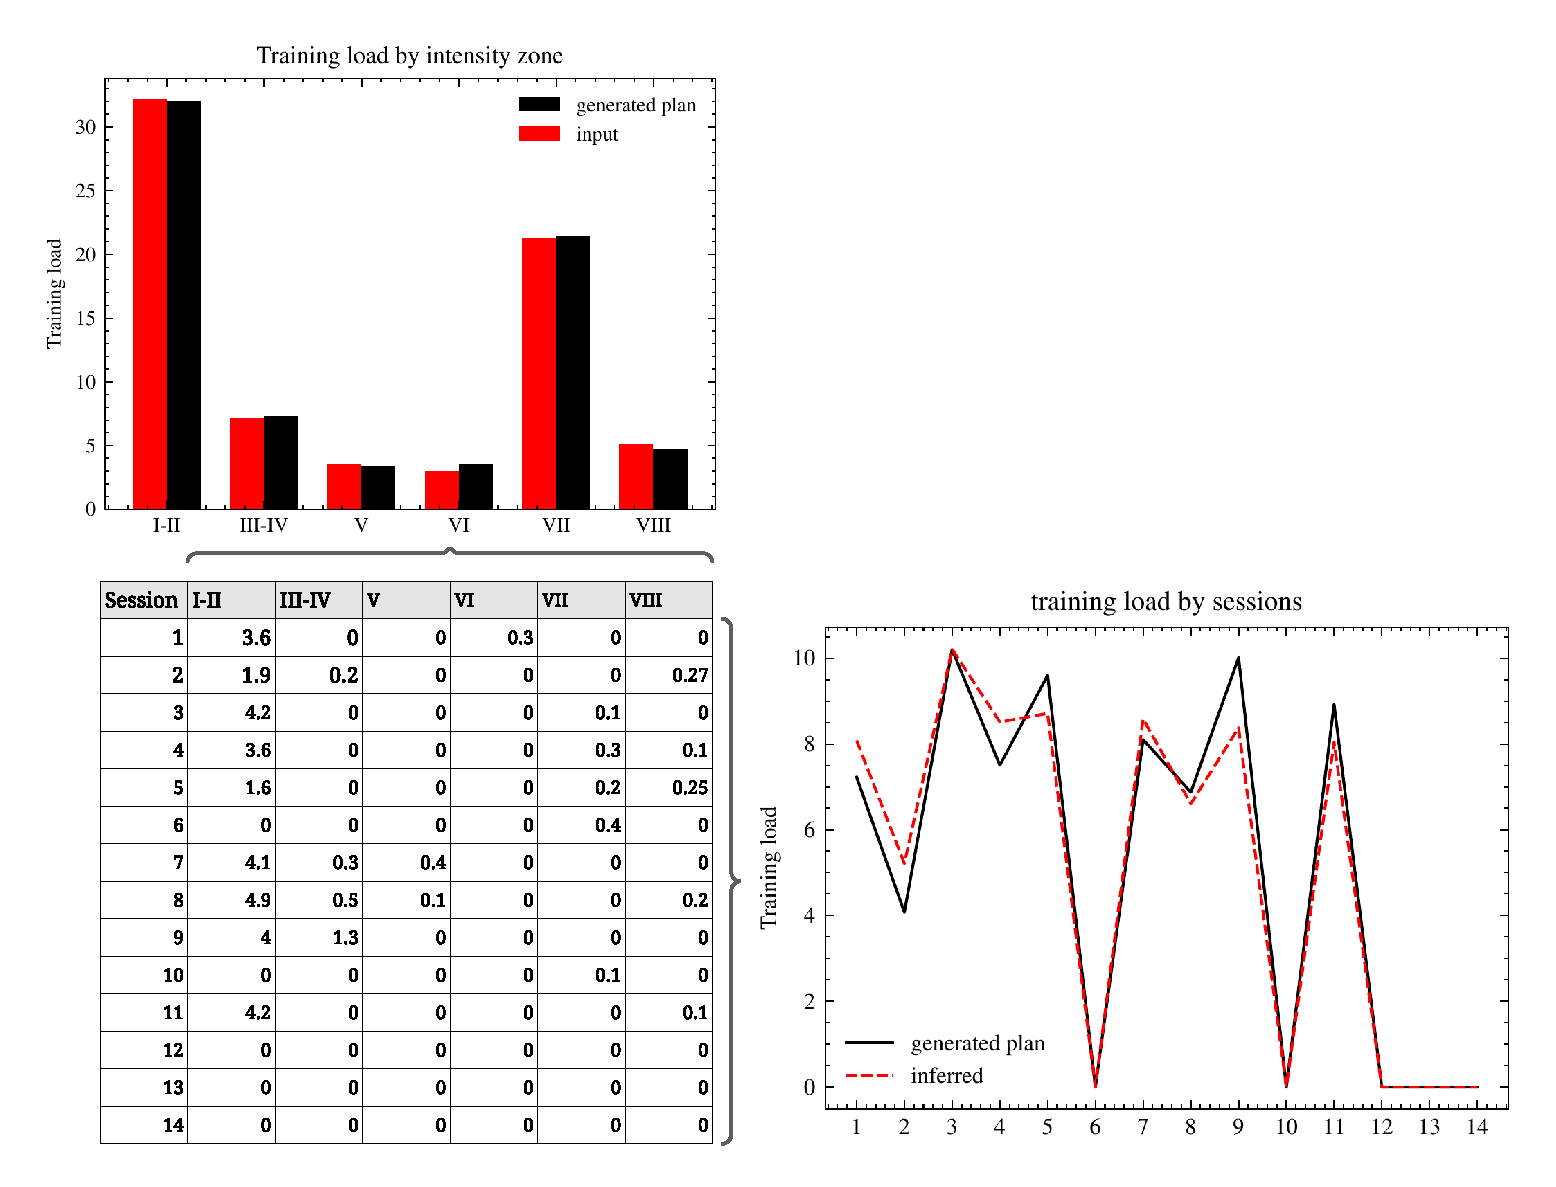
\includegraphics[width=1.0\linewidth]{chapters/figures/implementation_plots/GERT_evaluation.pdf}
    \caption{An illustration of the evaluation stage of GERT for a training plan over $e_Z$ (top), which ensures that the training plan has the same distribution of the intensity zones, and $e_D$ (right), which is responsible for the weekly distribution. Note that the inferred distribution is the output of the regressor model.}
    \label{fig:GERT_evaluation}
\end{figure}

When the fitness scores have been assigned, the termination criterion is checked.
The termination criterion is set such that the best sample of the population remains unchanged for a specified number of iterations.
The number of iterations is set as a hyperparameter in the model.
If the termination criterion is met, the training plan with the lowest fitness score is returned as output.
Otherwise, the worst scoring training plans are removed from the population until it has returned to the specified population size, and the next generation is started from the crossover stage.
% An example of the output can be seen in \cref{fig:GERT_output}

% \begin{figure}
%     \centering
%     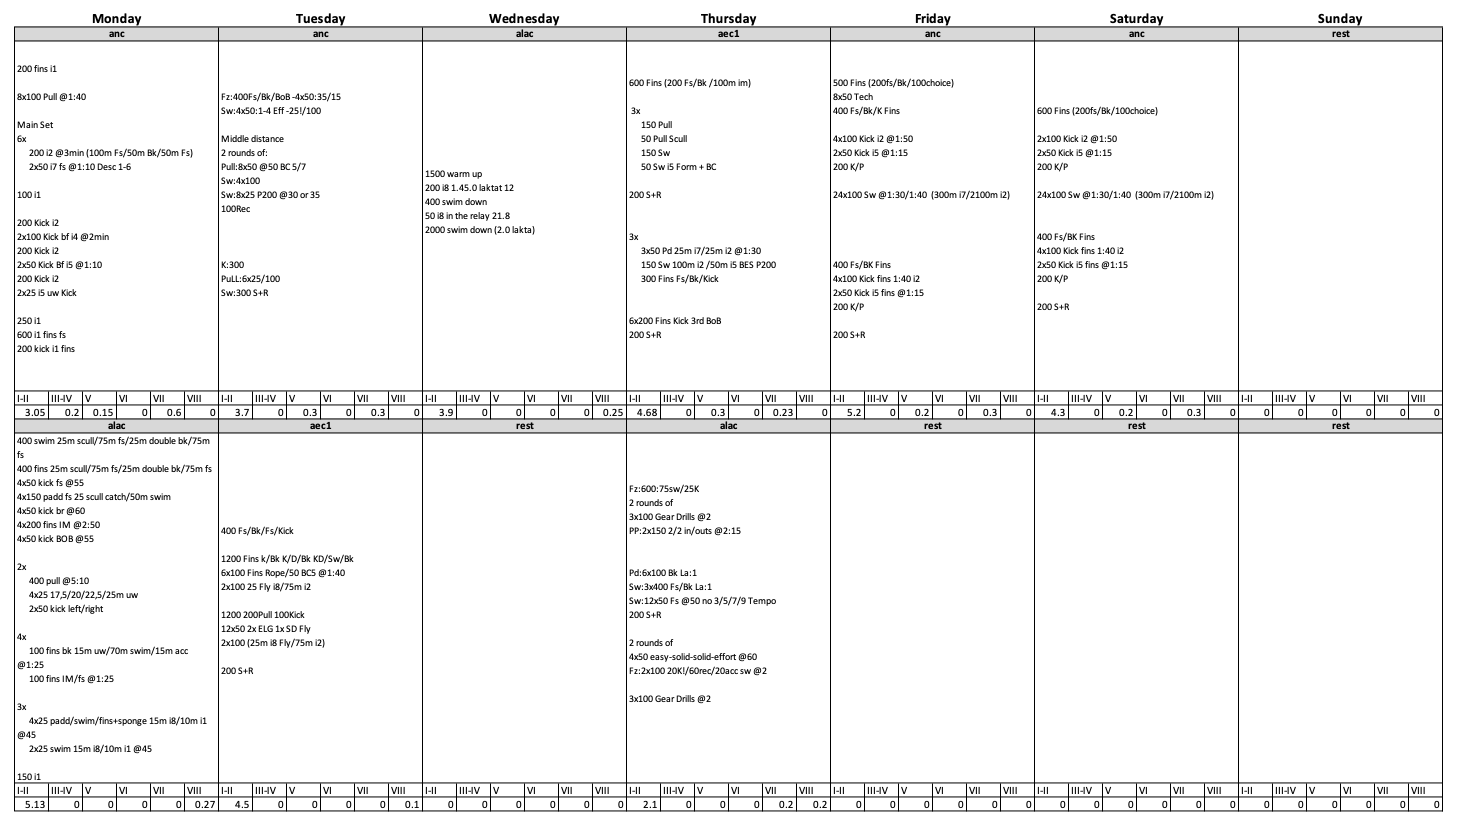
\includegraphics[width=1.0\linewidth]{chapters/figures/GERT_output.png}
%     \caption{An example of an output from the GERT model}
%     \label{fig:GERT_output}
% \end{figure}

The hyperparameters were tuned using five-fold cross-validation on the training data.
To reduce the number of values in the parameter grid, tuning was done in a two-step fashion.
During the first step of tuning, a coarser grid was constructed to find a range of interest.
The scope was then narrowed and the level of detail increased.
For the second step, all ranges were partitioned into 10 values of equal distance.
The parameters investigated can be seen in \cref{tab:param_range}.

\begin{table}
    \centering
    \begin{tabular}{@{}llll@{}}
    \toprule
    Parameter            & step 1 range         & step 2 range    & Final parameters \\ \midrule
    Population Size      & \{100, 500, 1000\}   & {[}300, 1000{]} & 750              \\
    Mutation Probability & \{0.02, 0.2, 0.5\}   & {[}0, 0.35{]}   & 0.1              \\
    Shuffle Probability  & \{0.02, 0.2, 0.5\}   & {[}0, 1{]}      & 0.25             \\
    Iterations           & \{10, 50, 100, 200\} & 12              & 12               \\ \bottomrule
    \end{tabular}
    \caption{A table showing the different values of parameters used in the tuning of GERT.}
    \label{tab:param_range}
\end{table}

A full evaluation of the parameter space was infeasible, since the evaluation of a parameter configuration took \SIrange{10}{50}{\minute}, depending on the population size.
Instead, the tuning during the second step was made by iteratively evaluating a subset of the parameters while the others were held fixed.

As can be seen in \cref{fig:param_search_cv_n_itter}, the parameter for the number of iterations before termination seemed to improve the score in the same way regardless of the values of the other parameters.
An elbow plot of the iterations was drawn and based on that plot a decision was made to fix the number of iterations to $12$ for all other runs.

\begin{figure}[ht]
    \centering
    \begin{subfigure}[t]{0.45\textwidth}
        \centering
        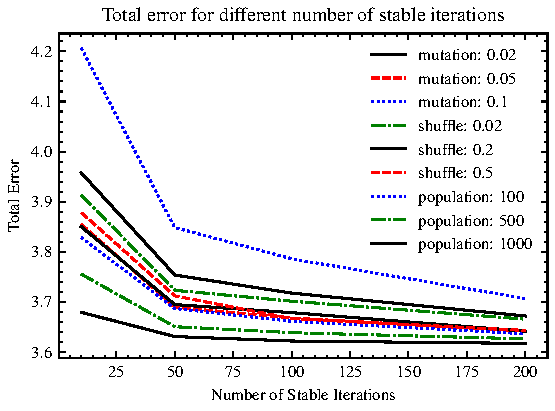
\includegraphics[width=\textwidth]{chapters/figures/iterations_plot_stage1.pdf}
        \captionsetup{width=.9\linewidth}
        \caption{The first stage of parameter tuning for the number of stable iterations. Scores go down similarly with an increased number of stable iterations, regardless of other parameters.}
    \end{subfigure}%
    ~ 
    \begin{subfigure}[t]{0.45\textwidth}
        \centering
        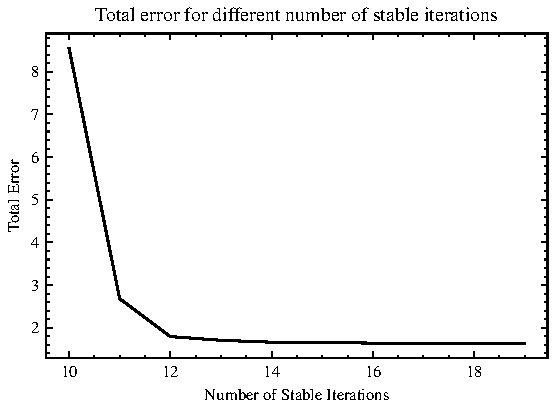
\includegraphics[width=\textwidth]{chapters/figures/iterations_plot.pdf}
        \captionsetup{width=.9\linewidth}
        \caption{Elbow plot for determining a cutoff for the number of stable iterations.}
    \end{subfigure}
    \caption{Plots from the tuning of the number of stable iterations hyperparameter.}
    \label{fig:param_search_cv_n_itter}
\end{figure}

The elbow criterion was used for both the number of iterations and the population size since these parameters affect the run-time which is desirable to keep low.
The elbow plot highlights a good trade-off between the diminishing return of performance and the increased time cost.
The elbow plot of the population size can be seen in \cref{fig:param_search_cv_population}.
Since the mutation probability and shuffle probability were thought to be highly dependent these were optimized together.
The results from the last step, when the process had converged, can be seen in \cref{fig:mutation_shuffle}.

\begin{figure*}[t!]
    \centering
    \begin{subfigure}[t]{0.45\textwidth}
        \centering
        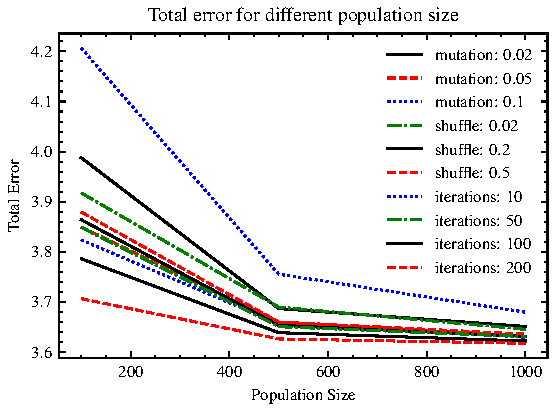
\includegraphics[width=\textwidth]{chapters/figures/implementation_plots/population_plot_stage1.pdf}
        \captionsetup{width=.9\linewidth}
        \caption{An elbow plot showing the results from the first stage of tuning for population size.}
    \end{subfigure}%
    ~ 
    \begin{subfigure}[t]{0.45\textwidth}
        \centering
        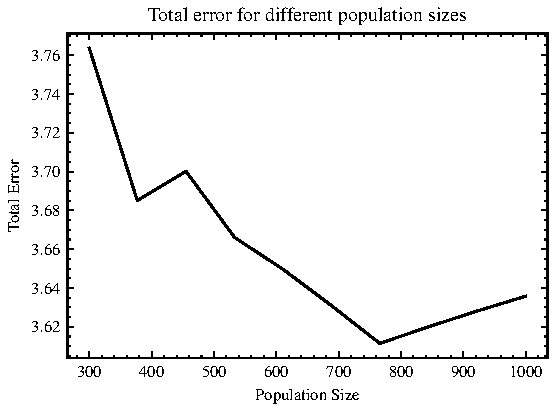
\includegraphics[width=\textwidth]{chapters/figures/population_plot.pdf}
        \captionsetup{width=.9\linewidth}
        \caption{A plot showing the score for different population sizes with the number of iterations set to $12$, shuffle probability set to $0.25$ and mutation probability set to $0.1$.}
    \end{subfigure}
    \caption{Illustrations of the search for optimal parameters for the GERT model. The plots are from the last iteration when the optimization reached a fixpoint.}
    \label{fig:param_search_cv_population}
\end{figure*}

\begin{figure}[ht]
    \centering
    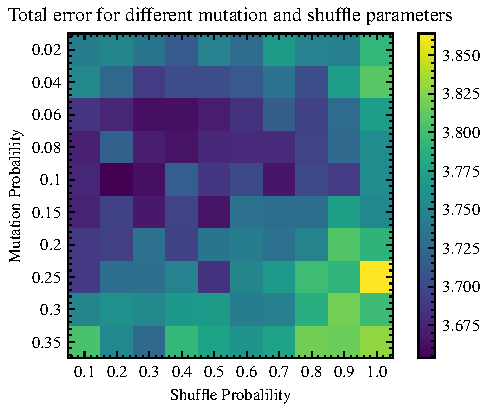
\includegraphics[width=0.5\textwidth]{chapters/figures/shuffle_mutation.pdf}
    \caption{A heat map of the results from the last stage of tuning the mutation and shuffle parameters.}
    \label{fig:mutation_shuffle}
\end{figure}

\section{Baseline models}
In this section, the models that were used in this thesis are described.

\subsection{Baseline KNN}
\label{sec:BKNN}
As a baseline, a nearest neighbour approach is taken.
The data set was split into a training and test set, see \cref{sec:data}.
Each week of training in \textit{weekly input}$_{train}$ was mapped into a vector space so that each dimension represented a feature of \textit{weekly input}, and associated with the corresponding training plan in \textit{detailed plans}$_{train}$.
To make predictions for the weeks in \textit{weekly input}$_{test}$ they were also mapped to the vector space.
For each week in \textit{weekly input}$_{test}$, the week in \textit{weekly input}$_{train}$ that was closest, measured in euclidean distance in the vector space, was identified. The corresponding training plan from \textit{detailed plans}$_{train}$ was returned as the prediction.

\subsection{Weekly Oracle}
\label{sec:WORC}
To get an upper limit for the performance of a method based on selecting a complete week, we introduce a \textit{Weekly Oracle} model.
The data is split into a train and test set as described in \cref{sec:data}.
The Weekly Oracle then has access to all the information in the test set and will choose the week of training from the training set that minimizes the loss function described in \cref{eq:loss_func}.
% This is also the same metric that is used in our planner GERT, that is described in \cref{sec:GERT}.
The Weekly Oracle can only pick an existing week, it cannot create new combinations.

\subsection{GERT Oracle}
\label{sec:GORC}
To get an upper bound on how well GERT would be able to perform given a perfect prediction of the weekly distribution, we implemented the GERT Oracle (GORC). 
GORC has the same prediction stage as the original GERT model, using the same hyperparameters and tuned values.
However, GORC has access to the \textit{actual} weekly distribution from the test set.
